\documentclass[twoside,11pt]{article}

% Any additional packages needed should be included after jmlr2e.
% Note that jmlr2e.sty includes epsfig, amssymb, natbib and graphicx,
% and defines many common macros, such as 'proof' and 'example'.
%
% It also sets the bibliographystyle to plainnat; for more information on
% natbib citation styles, see the natbib documentation, a copy of which
% is archived at http://www.jmlr.org/format/natbib.pdf

\usepackage{jmlr2e}
\usepackage{amsmath}

% Definitions of handy macros can go here

\newcommand{\dataset}{{\cal D}}
\newcommand{\fracpartial}[2]{\frac{\partial #1}{\partial  #2}}
\newcommand{\method}{{Deep MR}}

% Heading arguments are {volume}{year}{pages}{submitted}{published}{author-full-names}

\jmlrheading{1}{2000}{1-48}{4/00}{10/00}{Marina Meil\u{a} and Michael I. Jordan}

% Short headings should be running head and authors last names

\ShortHeadings{Deep Mendelian Randomization: Identifying and Verifying Genomic Deep Learning Models' Causal Knowledge}{Malina, Cizin, and Knowles}
\firstpageno{1}

\begin{document}

\title{Deep Mendelian Randomization: Identifying and Verifying Genomic Deep Learning Models' Causal Knowledge}

\author{\name Stephen Malina \email sdm2181@columbia.edu \\
       \AND
       \name Daniel Cizin \email todo@todo.edu \\
       \AND
       \name David A. Knowles \email dak2173@columbia.edu}
       

\editor{N/A}

\maketitle

\section{Outline}
\textbf{Why did I do this work?}

\begin{enumerate}
	\item Establish confidence in our models by validating they learn the qualitative relationships we're confident exist.
	\item Identify new potential qualitative relationships to investigate with experiments.
\end{enumerate}

\textbf{What work relates to ours?}
\begin{enumerate}
	\item Build on work applying DL models to epigenomic data. 
	\item Take a different approach than interpretability work like DeepLIFT analyzing what DL models learn. Tends to focus on individual samples or motifs rather than high-level relationships.
\end{enumerate}

\textbf{What does our method do?}
Identify and validate causal relationships learned by genomic DL models.

\textbf{What do our results mean?}
Finding that our models seem to learn the causal relationships we expect 

\textbf{What hypotheses did we test?} Whether our method could identify the right quantitative and qualitative causal relationships between epigenomic features.

\textbf{What did we learn?}

\textbf{What did/didn't work?}
In both simulation and real experiments, Deep MR mostly recovers the order of causal relationships but not the exact magnitude.

\textbf{What experiments did we do?}

\textbf{Why does it matter? Why should a reader care?}
Having a method that can verify genomic DL models learn the causal relationships we know exist would increase our confidence in them. 

\textbf{What work would we do next to expand on this project?}

\pagebreak

\paragraph{Guidance for the reader}
\subparagraph{Strategy} 
\subparagraph{Things to look out for}
\begin{itemize}
	\item Method's assumptions derived from traditional MR assumptions.
\end{itemize}

\subsection{Related Work}
In recent years, many researchers have applied deep learning to achieve impressive results at predicting transcriptomic features such as transcription factor (TF) binding~\cite{alipanahi2015predicting, zhou2015predicting}, chromatin accessibility~\cite{kelley2016basset, zhou2015predicting}, RNA binding protein (RBP) binding~\cite{zheng2018deep, zhang2019deepdrbp, koo2018inferring}, and DNA methylation states~\cite{angermueller2017deepcpg} from sequence and sometimes other auxiliary features. These models' ability to make reliable predictions of transcriptomic features on never-before-seen sequences may allow them to one day guide future investigation while saving valuable and scarce experimenter time. However, little work has been done to try and validate hypothesized causal relationships between phenomena using predictions from these models. 

In this work, we propose combining MR techniques with neural network generated data to test for a hypothesized causal relationship between transcription factor binding and chromatin accessibility. In doing so, we hope to enable trustworthy, interpretable estimates of causal effects, which may one day enable discoveries of new causal relationships from in-silico data. We test our method by estimating the postulated effect of CTCF binding on chromatin accessibility.

\paragraph{Summary}
\subparagraph{Experiments}
\begin{itemize}
	\item Test method on regression model trained on simulated data with known ground truth and simple generative process - two TFs where one's binding causes the other's.
	\item Applied method to two jointly trained models, one regression (BPNet) and one classification (DeepSEA), from the literature.
\end{itemize}

\subparagraph{Conclusions}


\section{Methods}%
\label{sec:methods}


\begin{figure*}[htpb]
    \centering
    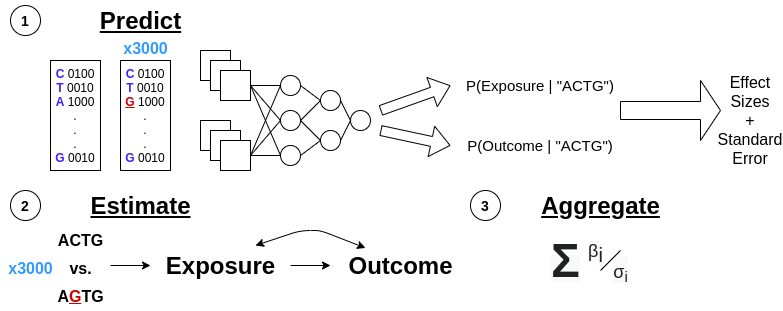
\includegraphics[width=.8\linewidth]{fig/model_overview.png}
    \vspace{-12pt}
    \caption{Graphical representation of Deep MR's high-level steps combining \textit{in silico} mutagenesis and MR (see Section \ref{sub:algo_overview}). \underline{Predict} corresponds to steps 1 through 4. \underline{Estimate} corresponds to step 5. \underline{Aggregate} corresponds to step 6}
    \vspace{-10pt}
    \label{fig:model_overview}
\end{figure*}

\subsection{Algorithm Overview}%
\label{sub:algo_overview}


Deep MR estimates causal effect sizes between variables predicted by a multi-task model. It takes a trained, calibrated (regression or classification) model that outputs predictive means and standard errors and a set of one-hot encoded sequences as input. In our case, the one-hot encoded sequence represents a sequence of nucleotides for the model to make predictions on.

Deep MR outputs local, sequence-specific causal effects and global, exposure/outcome-specific causal effects. It accomplishes this (see Figure~\ref{fig:model_overview} for a visual depiction) via the following steps for each exposure/outcome pair:
\begin{enumerate}
    \item Randomly sample sequences to predict exposure and outcome values for ``reference sequences''.
    \item Perform \textit{saturation in-silico mutagenesis} for each reference sequence to generate \( (\text{sequence\ length} \times \text{alphabet\ size} - 1) \) mutated sequences per reference sequence.
    \item For each set of pairs of mutant and reference sequences, generate predictive means and standard errors for exposure and outcome features.
    \item Generate \( (\text{sequence length} \times \text{alphabet size} - 1) \) \textit{effect sizes} by subtracting each reference sequence's predictive mean from the corresponding mutated sequences' predictive means. Also, compute the standard errors of these differences.
    \item Filter instruments by effect size based on a z-score threshold to only include those that are strongly associated with the exposure. \label{item:instr_filtering}
    \item Estimate a per-exposure, per-sequence region causal effect by running MR on the remaining effect sizes and their standard errors.
    \item Estimate overall per-exposure causal effects using a random effects meta-analysis.
\end{enumerate}

\subsection{Components}%
\label{sub:meth_components}

\subsubsection{Calibrated Model}%
\label{ssub:calibrated_model}

\subsubsection{MR Method}%
\label{ssub:mr_method}

\subsection{Key Assumptions}%
\label{sub:meth_key_assumptions}
\method\ relies on a few key assumptions regarding the DL model being used and the causal structure of the underlying data-generating process.

\subsubsection{Underlying Model Performance}%
\label{ssub:underlying_model_performance}
Because Deep MR uses variant effect estimates from a trained model rather than from real data as input to MR, the quality of its causal effect estimates is limited by the quality of the trained model. As a result, Deep MR works best when the trained model to which it's being applied achieves high accuracy on held-out test data.


\subsubsection{MR DAG Faithfulness}%
\label{ssub:mr_dag_faithfulness}
For MR to return unbiased causal effect estimates at the sequence region level, our underlying data-generating process and our model's proxy for it must both adhere to the three MR assumptions (\ref{par:rel_work_mr_assumptions}) and there must be a linear relationship between exposure and outcome features. In the statistical genetics setting, these assumptions can be justified in part by claims about the relationship between genotype, which is pre-natal, and potential confounders and phenotypes, both of which tend to be post-natal, assuming population structure is accounted for. We unfortunately cannot fall back on these justifications because they do not hold when looking at sequence-to-function relationships. Instead, we must re-examine each of these assumptions to determine whether they can be expected to hold. At a high level, assumption~\ref{item:mr_ass_2} is easy to satisfy because we can simply filter instruments based on their relationship to the exposure (see item~\ref{item:instr_filtering} in Section~\ref{sub:algo_overview}), whereas the unconfoundedness (assumption~\ref{item:mr_ass_1}), exclusion restriction (item~\ref{item:mr_ass_3}), and linearity assumptions have the potential to be violated.

\paragraph{Instruments Independent of Unobserved Confounders}%
\label{par:meth_instr_ind_conf}

Under classical MR assumptions, estimates will only be unbiased if all instruments are independent of any potential unobserved confounders. At the sequence-region level, potential unobserved confounders broadly fall into two categories: sequence-dependent and sequence-independent. Potential sequence-dependent unobserved confounders include other TFs or features which affect the exposure or outcome and which are affected by a mutation. In the case of an unobserved TF binding, this could manifest if a latent TF causally influences the exposure and the outcome. In this scenario, mutations which impact the latent TF's binding would also affect the exposure and therefore prevent this specific mutation from being filtered out during step~\ref{item:instr_filtering}. Despite appearing as valid instruments, such mutations would clearly violate the instrument independent of unobserved confounders criterion and therefore bias classical MR estimates. Another potential sequence-dependent confounder would be an uncorrected assay bias such as GC-bias. GC-bias pushes estimates of read counts higher in regions with higher-than-average GC-content, thereby biasing models to systematically predict higher values for such regions. In MR terms, GC content acts as an unobserved confounder which causes mutations from A/T to C/G to incorrectly increase predicted exposure and/or outcome values. We don't have plausible examples of sequence-dependent confounding, but explore the effects of both types on the quality of our sequence-region level causal effect estimates in our simulation experiment nonetheless (TODO: ref).


\noindent TODO: add more to this section and decide whether to move some of it to discussion.\\
TODO: what are examples of potential non-sequence dependent unobserved confounders? We consider this sequence-independent because although it depends on sequence content, its effect should be almost entirely independent 

\paragraph{Exclusion Restriction}
The exclusion restriction assumption requires all influence of an instrument, in our case a mutation, on the outcome to be mediated by the exposure. Thus, the latent TF confounder example given above violates the exclusion restriction assumption. The latent TF also influences the outcome variable, so mutations that influence the latent TF would also influence the outcome via the latent TF, i.e. through a pathway not mediated by the exposure. In classical MR, this violation would be enough to bias our causal effect estimates. However, the MR Egger method provides some additional conditions under which unbiased estimates are possible in the presence of one or more exclusion restriction violations. MR Egger is designed to furnish unbiased estimates of causal effects in the presence of exclusion-restriction violations as long as these violations satisfy the assumption that instrument strength for invalid instruments is independent of the magnitude of the direct effect (InSIDE assumption).

\paragraph{Local Linearity}%
\label{par:meth_local_linearity}
As discussed in Section~\ref{par:rel_work_mr_assumptions}, MR correctly estimates causal effects when all relationships -- instrument to exposure and exposure to outcome -- are linear. However, in functional genomics settings, the relationship between phenotypes can be non-linear. For example, in the case of strong TF binding cooperativity, knocking out one TF's binding will knock out the other's entirely, violating linearity. Fortunately, in our application, we only require the weaker condition of local linearity to hold in order for our method to work. Concretely, because each of our effect sizes is derived from the predicted effect of a single point mutation on the exposure/outcome phenotypes, our method works as long as the relationships between exposure and outcome predictions stays linear within the local neighborhood of the initial values.
















\section{Experiments}
\subsection{Simulation}

\subsection{}

\section{Discussion}
\subsection{Challenges}
\subsubsection{Mendelian Randomization requires strong assumptions}

\subsubsection{Obtaining calibrated standard error estimates for sequence-level causal effect estimates}

\subsubsection{Deep MR's accuracy is limited by the accuracy of the underlying model}





% Acknowledgements should go at the end, before appendices and references

% Manual newpage inserted to improve layout of sample file - not
% needed in general before appendices/bibliography.

\newpage

\appendix
\section*{Appendix A.}
\label{sec:appendix_a}

\subsection*{Computing Counts}%
\label{sub:app_a_computing_counts}






\vskip 0.2in
\bibliography{bib}

\end{document}

%%% Local Variables:
%%% mode: latex
%%% TeX-master: t
%%% End:
